\chapter{Background}\label{ch2:background}

\section{Geothermal Systems}\label{ch2:geosys}
\subsection{Heat Origins}
\subsubsection{Accretion}
The story of geothermal energy begins with the birth of planet Earth. Approximately 4.56 billion years ago \citep{allegre_age_1995, patterson_age_1956}, the Earth coalesced as a molten body heated by repeated impacts with objects in the early solar system like the planetesimal impact responsible for the formation of the Moon \citep{stevenson_origin_2014}. Over tens of millions of years, the Earth compacted, cooled, and differentiated, settling into the familiar layered structure of a solid inner core, liquid outer core, viscous mantle, and outermost brittle crust \citep[~p. 7]{press_understanding_2004}. The intense heat from that early accretionary history remains concentrated in the core, where temperatures - a matter of continued scientific inquiry - fall in the range of 6000±500 K \citep[~p. 372]{fowler_solid_2005}. Present day heat flux estimates for the whole Earth amount to 87 mW/m\textsuperscript{2}, \texttt{\char`\~}60\% of which flows through conductive and convective pathways from the deep interior to outermost crust \citep{stein_heat_1995}. Diffuse conductive heat transfer occurs everywhere across of the Earth’s surface, but heat flow concentrates along tectonic plate boundaries. In fact, the subduction-sourced volcanoes that ring the Pacific Ocean, divergent zones at the mid-ocean ridges and East African rift, and major strike-slip boundaries like the San Andreas fault zone all mark locations where focused heat anomalies are already being tapped by geothermal installations \citep[~p. 16]{dipippo_geothermal_2012}.
\subsubsection{Radioactive Decay}
The second major source of heat within the Earth is the decay of radioactive isotopes. Early radioactive heating included radioisotopes with short half-lives like Aluminum-26 and Hafnium-182, which are now no longer present \citep[~p. 16]{glassley_geothermal_2015}. Among the radioactive elements contributing the most to heating the crust today are uranium (U), thorium (Th), rubidium (Rb), and potassium (K) \citep[~p. 17]{glassley_geothermal_2015}. The decay of these and other elements accounts for 40\% of the crustal thermal budget \citep{stein_heat_1995}. But element abundances are not distributed uniformly throughout the crust. On average, continental crust, particularly the upper continental crust, has significantly higher concentrations of U, Th, and K radioactive elements compared to oceanic crust, and both types of crust are 1-2 orders of magnitude more enriched than the mantle \citep[~p. 276]{fowler_solid_2005}. This relationship holds for representative igneous rock types; granite generates more heat than basalt, and both out-produce ultramafic rocks like peridotites \citep[~p. 276]{fowler_solid_2005}.
\subsection{Heat Measurements}
\subsubsection{Geothermal Gradient}
Average subsurface conditions show a steady increase in temperature with depth, commonly referred to as the geothermal gradient, sustained by the flow of original accretionary heat and generated radioactive heat. On average, the gradient for continental crust is \texttt{\char`\~}30\textdegree C/km \citep[~p. 209]{press_understanding_2004}. However, deviations from this value are common and reflect the complexity of the rock record in an area. The crust comprises a distinct set of layers, or strata, that vary in composition and rock type. Unlike the aforementioned igneous formations that can be relatively homogeneous, surface processes mix sediments from a variety of original source rocks, sometimes sorting them well and sometimes not, before they get deposited and indurated into sedimentary formations \citep[~p. 164-168]{press_understanding_2004}. Alteration from fluids, heat, and pressure can then modify the composition of these rocks, causing constituent minerals to change form and arrangement to create metamorphic rocks \citep[~p. 195-205]{press_understanding_2004}. The spatial and depth variations in these formations create subsurface compositional heterogeneity, directly reflected in rock properties. Thermal conductivity, specifically the ability to move deep-sourced heat to shallower depths, and radioactive element abundance, or the ability to generate additional heat in situ, can therefore vary in all directions in the subsurface. Thermal heterogeneity can be further compounded by anomalies created from salt movement \citep[~p. 164-168]{press_understanding_2004}, magmatic intrusions, or global tectonic processes. It therefore takes a good understanding of the geology and geologic history to determine the geothermal gradient of a region.
\subsubsection{Heat Flow}
Fundamentally, heat moves from hot to cold (Second Law of Thermodynamics) at a rate that linearly scales with the thermal gradient. Simple, one-dimensional thermal conduction can be characterized by the relationship \citep[~p. 270]{fowler_solid_2005}:
\begin{equation}\label{eq:conduction}
q = -k \frac{\nabla T}{x}
\end{equation}
where q is heat flux, or heat flow per unit time per unit area, with S.I. units of \(Wm^{-2}\). Heat flux depends on the gradient of temperature (T), the distance over which conduction takes place (x), and the thermal conductivity (k), that is, the ability of material to conduct heat. Different rock types have different values of k, e.g., sandstone varies from 1.60-2.10 \(W/m^\circ C\) while granite tends to be higher with values ranging from 1.73-3.98 \(W/m^\circ C\) \citep[~p. 30]{dipippo_geothermal_2012}. Feldspars and quartz exhibit significant (up to 3x) differences in k values. As the most abundant minerals in crustal rocks, their relative fractions will strongly influence the thermal conductivity of a formation \citep[~p. 22]{glassley_geothermal_2015}. Regardless, minerals tend to be relatively poor thermal conductors compared to other materials like aluminum (210 \(W/m^\circ C\)) and iron (73 \(W/m^\circ C\)), making conduction a slow method of crustal heat transmission \citep[~p. 23]{dipippo_geothermal_2012}.

Conduction dominates on local scales in the crust, while convection is the primary means of heat transfer on global, tectonic scales. Even in its two-dimensional form with no internal heat generation, the equation governing convection is much more complex than for conduction \citep[~p. 355]{lowrie_fundamentals_2007}:
\begin{equation}\label{eq:convection}
\frac{\partial T}{\partial t} = \left (\frac{k}{\rho * c_P}\right)\left (\frac{\partial ^2T}{\partial x^2}+\frac{\partial ^2T}{\partial z^2}\right)-u_x\frac{\partial T}{\partial x}-u_z\frac{\partial T}{\partial z}
\end{equation}
where \textbf{u} = \(( u_x, u_z)\) is the velocity of the fluid, \(\rho\) is the material density, and \(c_P\) is the specific heat, which defines the amount of heat necessary to raise 1 kg of that material by 1\(^\circ C\) Convention combines heat transfer from conduction with mass movement. Since the minerals are relatively poor conductors of heat, the combined effects of lower viscosity and thermal expansion – as seen near the core-mantle boundary – and gravitational forces that create buoyancy effects, all create the right conditions for convective flow, e.g. within the mantle \citep[~p. 25]{glassley_geothermal_2015}. Mantle convection is responsible for the high heat flow values observed at crustal plate boundaries like mid-ocean ridges, as well as intraplate diapiric hot spots underlying Hawaii, Yellowstone, and a number of other locations around the world.  Smaller-scale convection also takes place at subduction zones where the material from the down-diving plate melts at lower temperatures with the presence of water, migrates upwards, and forms volcanic arcs on the surface as observed in Japan, Indonesia, and the Pacific Northwest of the U.S. \citep[~p. 31-33]{press_understanding_2004} – all locations with geothermal potential.

Heat flow measurements capture the flux of heat through the Earth’s surface as a result of these and other complex processes taking place in the subsurface. In this respect, it serves as a simpler and more accessible metric for local or regional heat potential than the more sparsely-measured and less well-constrained geothermal gradient. Today, high-quality heat flow measurements can be obtained in marine conditions, on continental margins, on mid-ocean ridges, and from the multitude wells drilled by the oil \& gas industry, supporting the creation of large heat flow data sets like the New Global Heat Flow database \citep{lucazeau_analysis_2019}. As Figure \ref{fig:heatflow} shows, data from these collections can be gridded to create spectacular maps of heat flow variations around the world. These maps offer a good starting point for quickly targeting where the greatest geothermal potential exists at the regional or “play” scale, which can then be further refined through additional methods (see Section \ref{ch2:geoexp}).
\begin{figure}[h!]
\centering
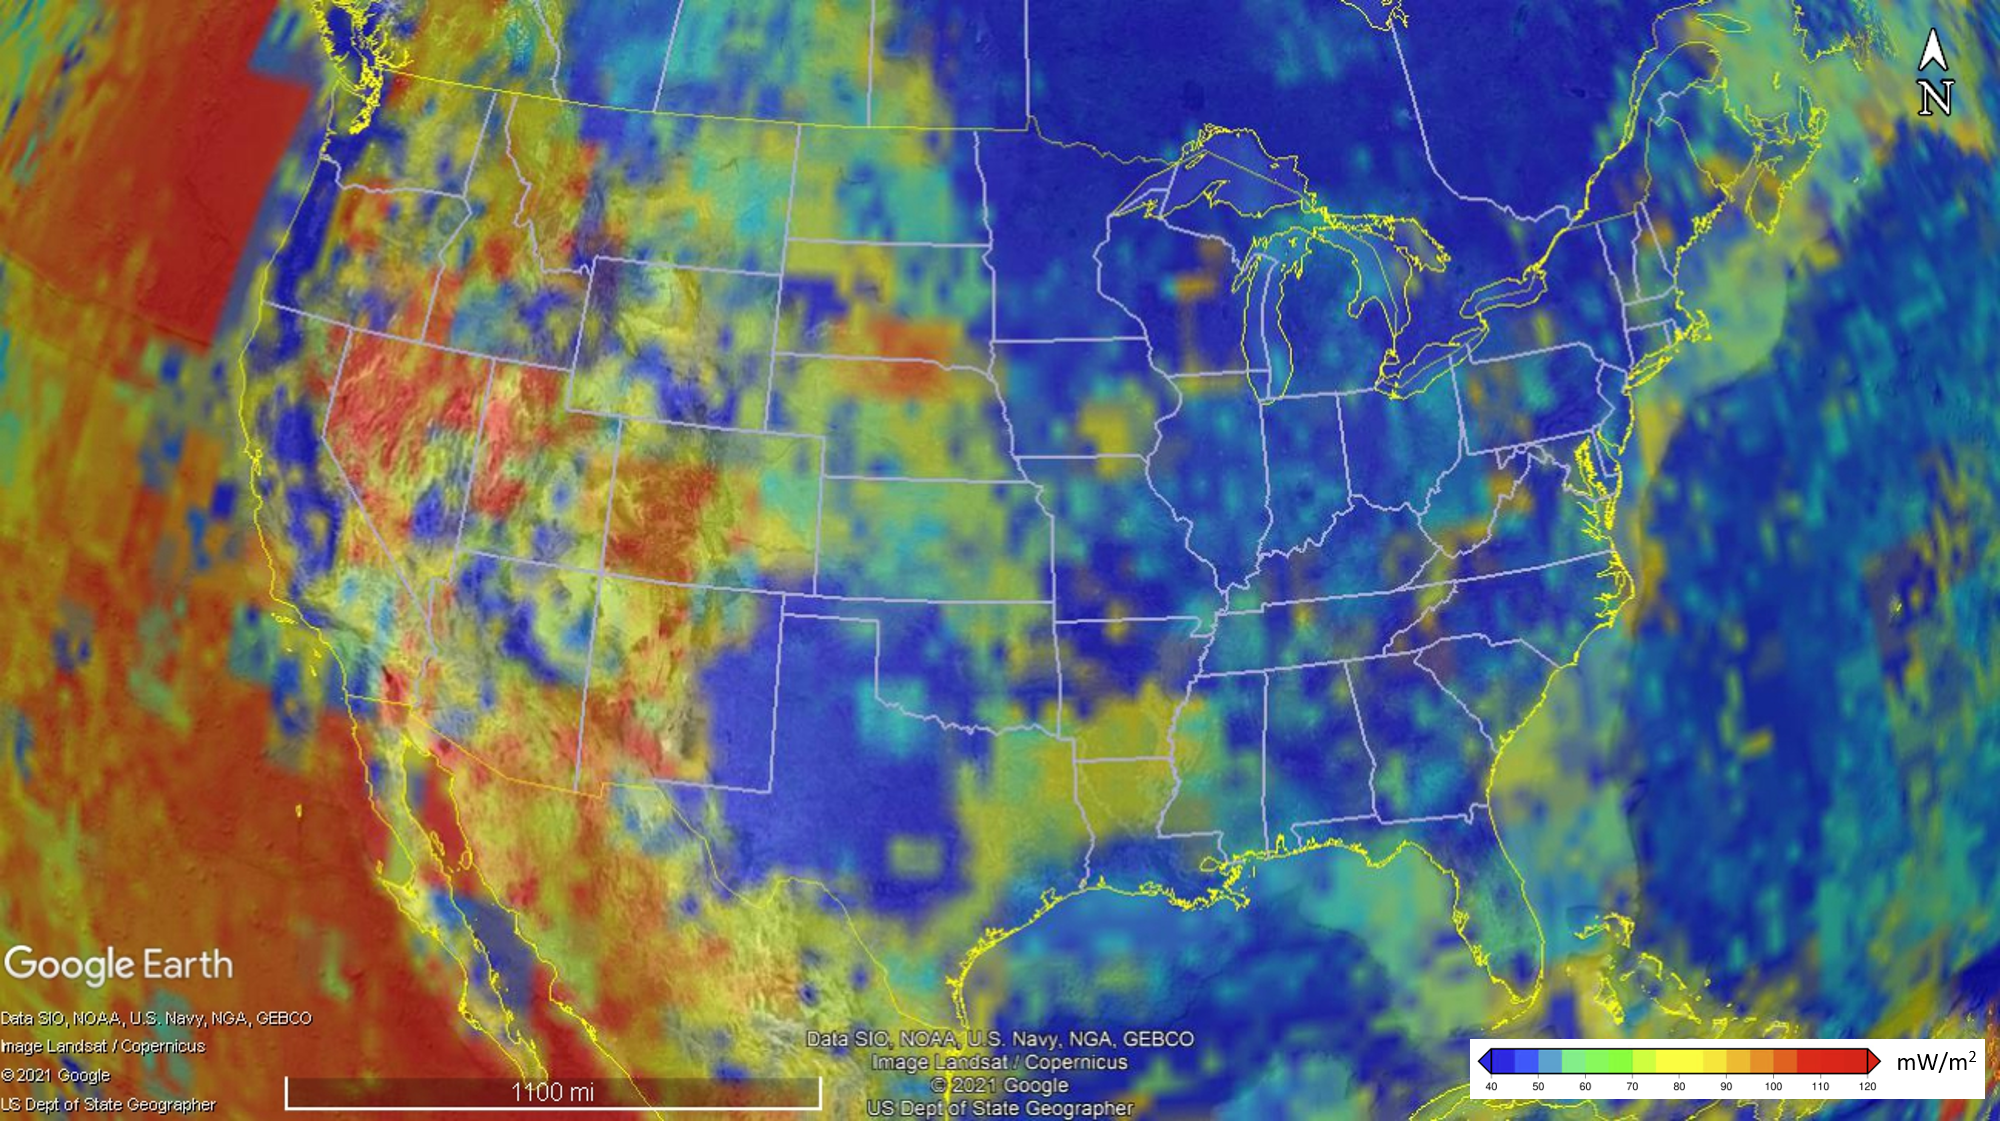
\includegraphics[scale=0.45]{Figure-HeatFlowMap}
\caption[Heat flow across the continental U.S.]{Heat flow estimates for the continental United States, plotted in Google Earth with data layer from \protect\citep{lucazeau_analysis_2019}}
\label{fig:heatflow}
\end{figure}
\subsection{System Fundamentals}
The conventional concept of a geothermal system consists of five key entities \citep[~p. 9]{dipippo_geothermal_2012}:
\renewcommand{\labelenumi}{\roman{enumi}}
\begin{enumerate}
   \item Heat source of significant size and temperature
   \item Permeability, typically in the form of a fracture network within crystalline rock
   \item Ample volume of working fluids, e.g. water from precipitation and drainage
   \item Impermeable sealing layer
   \item Consistent, reliable fluid recharge
\end{enumerate}

\subsubsection{Hydrothermal Systems}
If naturally present, the combination of these five elements defines a hydrothermal system. As water percolates down, captures heat from the permeable thermal reservoir, and gets trapped beneath the sealing caprock, a small fraction of the resource can escape to the surface to produce distinctive geothermal manifestations like fumaroles, hot pools, geysers, mud pots, and discolored or altered rocks (Figures \ref{fig:lassen-geysers} and \ref{fig:lassen-mudpot}). These features are strong indicators of hydrothermal resources at depth.
\begin{figure}[h!]
\centering
\includegraphics[scale=.84]{Figure-Lassen-geysers3}
\caption[Terminal Geyser, Lassen National Park]{Terminal Geyser, Lassen National Park, California. Photo credit: Author}
\label{fig:lassen-geysers}
\end{figure}
\begin{figure}[htbp]
\centering
\includegraphics[scale=0.27]{Figure-Lassen-mudpot}
\caption[Mud pot, Lassen National Park]{Active mud pot and ground staining on the bank of Boiling Springs Lake, Lassen National Park, California. Photo credit: Author}
\label{fig:lassen-mudpot}
\end{figure}
The original geothermal systems exploited by mankind for millennia are hydrothermal systems. Artifacts show proto-Native American use of hydrothermal waters for cleaning and health restoration over 10,000 years ago \citep{doe_history_2021}. The importance of geothermal hot springs for Roman, Japanese, Chinese, and Ottoman baths is also well-established in the historical record \citep{lund_characteristics_2007}. Industrial use began in the 1800s with chemical extraction from geothermal steam, pools, and deposits in Larderello, Italy \citep[~p. 251]{dipippo_geothermal_2012}. \acrlong{gdh} (\acrshort{gdh}), or large-scale heating of residences and businesses using geothermal-produced fluids, was pioneered in Chaudes-Aigues, France in the 1300s and first introduced to the United States in 1892 with an installation in Boise, Idaho \citep{lund_characteristics_2007}.

These few examples capture some of the many potential opportunities for low-temperature (<90\(^\circ C\)) and medium-temperature (<150\(^\circ C\)) geothermal resource use, even beyond hydrothermal systems. GDH can help meet building and water temperature needs, and agriculture, textiles, paper, chemicals, and even the food industry can also benefit from access to low-temperature geothermal fluids \citep{doe_low_2021,liu_overview_2015}. Interest has led to funding from agencies like the \acrlong{gto} (\acrshort{gto}) within the \acrlong{doe} (\acrshort{doe}); a grant was recently awarded to Cornell University in support of piloting a deep direct-use project to provide baseload heating for the university campus supporting peak demand during cold upstate New York winter months  \citep{hamm_geothermal_2021,tester_integrating_2015}.

The topic of this thesis instead concerns the use of moderate- to high-temperature geothermal for power generation. The first example of geothermal power production came from Italian experiments in 1904, and the first commercial plant went online in Larderello, Italy in 1914 \citep[~p. 251]{dipippo_geothermal_2012}. Geothermal-generated electricity made its debut in the United States with the development of The Geysers field beginning in 1960 \citep{tester_future_2006}. Hydrothermal plants quickly appeared in New Zealand, Japan, Iceland, Indonesia, Kenya, Philippines and elsewhere throughout the 1970s-1980s, with continued growth through to present-day \citep{lund_characteristics_2007}. 2020 statistics from the \acrlong{irena} (\acrshort{irena}) place the United States as world leader in geothermal installed capacity (2587 MW), followed by Indonesia (2131 MW) and Philippines (1928 MW) \citep{irena_country_2021} (Figure \ref{fig:irena-rank}). 

\begin{figure}[htbp]
\centering
\includegraphics[scale=.45]{Figure-IRENA_Rankings}
\caption[Country rankings, installed geothermal capacity ]{Countries ranked by installed geothermal capacity, from \protect\citep{irena_country_2021}}
\label{fig:irena-rank}
\end{figure}

A comprehensive assessment of moderate and high-temperature \acrlong{kgra} (\acrshort{kgra}) by the \acrlong{usgs} (\acrshort{usgs}) determined the U.S. has conventional geothermal (hydrothermal) power generation potential of \texttt{\char`\~}9,000 MWe, and an additional \texttt{\char`\~}30,000 MWe potential exists in undiscovered resources \citep{williams_assessment_2008}. The recent DOE GeoVision study notes hydrothermal potential in Alaska and Hawaii alone are \texttt{\char`\~}8000 MWe due to their unique tectonic environments (Aleutian subduction zone and Hawaiian hot spot, respectively), and high-case model estimates for the continental U.S. forecast an installed capacity of \texttt{\char`\~}16.5 GW by 2050 for known and unknown hydrothermal resources \citep{augustine_geovision_2019,hamm_overview_2019}.

\subsubsection{Enhanced Geothermal Systems}

\section{Geothermal Exploration}\label{ch2:geoexp}
\subsection{System Type}
\subsubsection{Direct Use}
\subsubsection{Conventional}
\subsubsection{Enhanced}
\subsection{Strategies}
\subsubsection{Play Fairway Analysis}
\subsubsection{Unsupervised Machine Learning}
\subsubsection{Supervised Machine Learning}
\subsection{Uncertainties}
\subsubsection{Important Indicators}
\subsubsection{Data Coverage}
\subsubsection{Measurement Uncertainty}
\section{Power Generation}\label{ch2:elec}
\subsection{Surface}
\subsubsection{Dry Steam}
\subsubsection{Flash}
\subsubsection{Binary Cycle}
\subsection{Subsurface}
\subsubsection{Natural Drive}
\subsubsection{Hard Rock EGS}
\subsubsection{Stratigraphic EGS}
\subsubsection{Advanced Closed Loop}
\subsection{Uncertainties}
blah blah blah

\section{Cost Modeling}\label{ch2:costmod}
\subsection{MIT Energy Lab}
\subsection{Cornell Lab}
\subsection{GETEM/SAM}
blah blah blah

\section{Case Study}\label{ch2:case}
\subsection{New Mexico Geothermal}
\subsection{Southwest NM Study Area}
\subsection{Lightning Dock Power Plant}
blah blah blah

%% EXAMPLES %%

%section~\ref{ch1:sec}.

%\footnote{Here is a sample footnote referencing figures~\ref{arm:fig1}
%and~\ref{arm:fig2}.}  

% This is an example of how you would use tgrind to include an example
% of source code; it is commented out in this template since the code
% example file does not exist. To use it, you need to remove the '%' on the
% beginning of the line, and insert your own information in the call.
%
%\tagrind[htbp]{code/pmn.s.tex}{Code sample}{opt:pmn}

%\subsection{Subsection with list}
%\begin{enumerate}
%  \item Item 1.
%  \item Item 2.
%  \item Item 3.
%\end{enumerate}

%This is done by using some combination of
%\begin{eqnarray*}
%a_i & = & a_j + a_k \\
%a_i & = & 2a_j + a_k \\
%a_i & = & 4a_j + a_k \\
%a_i & = & 8a_j + a_k \\
%a_i & = & a_j - a_k \\
%a_i & = & a_j \ll m \mbox{shift}
%\end{eqnarray*}

%instead of the multiplication.  For example, you could use:
%\begin{eqnarray*}
%r & = & 4s + s\\
%r & = & r + r
%\end{eqnarray*}
%Or by xx:
%\begin{eqnarray*}
%t & = & 2s + s \\
%r & = & 2t + s \\
%r & = & 8r + t
%\end{eqnarray*}
